 \documentclass[12pt]{article}
 \usepackage{graphicx}
 \usepackage{multirow}
 \usepackage{amsmath}
 \usepackage{fullpage}
 \usepackage{times}
 \setlength\parindent{0pt}
 \setlength\parskip{12pt}

 \usepackage{bigstrut}

 \begin{document}

 {\sffamily
 \begin{tabular}{lll}
 \multirow{8}{1in}{\includegraphics[width=1in]{ach.png}} & &\\%\multirow{9}{1in}{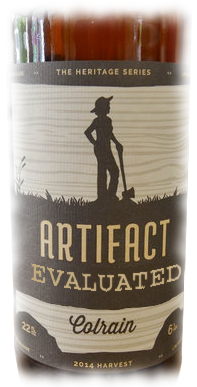
\includegraphics[width=1in]{eval.png}}\\
 & &\\
 & \large{\em CONFIDENTIAL COMMITTEE MATERIALS} &\\
 & &\\
 & \textbf{\LARGE{SIGBOVIK 2016 Artifact Evaluation}}& \\
 & &\\
 & \Large{Paper 10: Pittsburgh is a Grid} & \\
 &\\
 \vspace{1em}\\
 \hline
 \end{tabular}}
 \vspace{2em}
 \thispagestyle{empty}


\textbf{Claim 1:}  \textit{The authors claim to have constructed a Pittsburgh-gridding algorithm in Standard ML.}

\textbf{EVALUATION OF CLAIM:}
  The provided code was not a Standard ML program, but was clearly
  an attempt at producing one. After extensive consultation with local French experts, the committee
  managed to extract a Standard ML program from the provided code, and proceeded under the
  assumption that this is what was intended.

  In the future, we implore the author to provide proper Standard ML programs with their submis-
  sions. If the author is incapable of learning Standard ML on their own, we recommend the course
  15-150.

\textbf{Claim 2:}  \textit{The authors claim that Pittsburgh is a grid.}

\textbf{EVALUATION OF CLAIM:}
  The evaluation committee has confirmed that submission contains
  grid-like shapes, but has failed to verify equivalent claims about Pittsburgh proper. We sent an
  undergraduate to search for grids, who then got stuck in an infinite loop on Boulevard of the Allies
  and nearly starved to death before being rescued by a crack team of topologists.

  Before recklessly endangering Danny in this way again, we kindly suggest you evaluate your own
  work more closely before thrusting it upon this already-overburdened committee. In particular, it
  is well-known that all graphs form grids under the appropriate rounding conditions, and thus the
  veracity of your result is under question. As is the applicability, since the Peduto administration is
  a vocal opponent of the corn industry in general, and these ``kernel methods'' in particular.

\textbf{Claim 3:}  \textit{The authors claim an inability to perform integrals.}

\textbf{EVALUATION OF CLAIM:}
  This claim is pretty obvious, if you ask me. The authors did not even
  consider the numerical stability concerns inherent to all numerical integration methods, let alone
  give a convincing argument why their methods were stable. Instead of drawing on the extensive
  results in computer algebra, widely available in commercial systems such a Mathematica, they
  snobbishly implemented everything from scratch with inferior results. Like come on man, not even Euler integration? Runge and Kutta are spinning in their graves.

\textbf{OVERALL EVALUATION:}
 Well, the PC told us to go easy on this one as a personal favor, so
 with great remorse we give this submission our approval. Pittsburgh is a grid, no matter how many
 weeks Danny spent on life support in UPMC Presby.

\textbf{ADDITIONAL COMMENTS:}
\begin{itemize}
\item While evaluations are normally provided as a free service by the organizers of the conference
and their students, the medical expenses associated with this evaluation were well in excess
of \$100,000. This is partially covered by the author's travel allowance, but he will be billed
the difference.

\item You should seriously take 15-150. In all my years of teaching I have never seen such hideous
SML code, not from the worst students, not even from the French. What kind of animal calls
\texttt{float\_to\_int} over and over again on the same argument instead of let-binding like a
civilized human being? And how lazy do you have to be to leave commented-out code in a
conference submission? If you’re going to insist on programming in French, at least tell us
about your eclectic choice in graphing libraries. The quadtrees also seemed a bit excessive.

\item Minus one style point for lines in excess of 80 characters
\end{itemize}
 \end{document}
